\documentclass[a4paper, 12pt]{article}	
\usepackage{hyperref}
\usepackage{amsmath}
\usepackage{color}
\usepackage{graphicx}
% This is just one of many available `classes'
\begin{document}
\title{My First LaTeX Document!}
\date{01/11/2013}
\author{Charlie Rahal\\
Department of Economics,\\
UoB,\\
Birmingham.\\
\href{mailto:CXR828@bham.ac.uk}{cxr828 at bham.ac.uk}}
\maketitle
\begin{abstract}
This is an abstract which details the creation of our first adventures with \LaTeX.
\end{abstract}
% Begin/end document prefix and suffix all documents.
\tableofcontents

\newpage
\section{Text and Characters}
Hello World!\\

This is an % stupid
% Better: instructive <----
example: Supercal%
ifragilist%
icexpialidocious

\subsection{Bold}
Our first attempt at writing \textbf{SOMETHING IN BOLD!}
\subsection{Italics}
\subsubsection{textit}
\textit{This is written using textit}
\subsubsection{emph}
\emph{This is written using emph}
\subsection{Typewritter}
\texttt{This is in typewritter font}
\subsection{Underline}
\underline{This is underlined}
\subsection{Colors}
\colorbox{red}{TEST}
\fcolorbox{red}{green}{TEST}
\subsection{Lists}
\newpage
\section{The Beauty of Mathematics in LATEX}
\begin{equation}
a^2+b^2=c^2
\end{equation}
\begin{equation}
\lim_{n \to \infty}
\sum_{k=1}^n \frac{1}{k^2}
=\frac{\pi^2}{6}
\end{equation}
\begin{equation}
\begin{matrix}
1 & 2 & 3 & 4 & 5 \\
6 & 7 & 8 & 9 & 10 \\
11 & 12 & 13 & 14 & 15\\
16 & 17 & 18 & 19 & 20\\ 
21 & 22 & 23 & 24 & 25 \\
\end{matrix} \qquad =
\begin{bmatrix}
p_{11} & p_{12} & \ldots
& p_{1n} \\
p_{21} & p_{22} & \ldots
& p_{2n} \\
\vdots & \vdots & \ddots
& \vdots \\
p_{m1} & p_{m2} & \ldots
& p_{mn}
\end{bmatrix}
\end{equation}
\section{Figures}
\begin{figure}[!ht]
\begin{center}
\caption{\color{red}\textbf{Cat with monocle}}
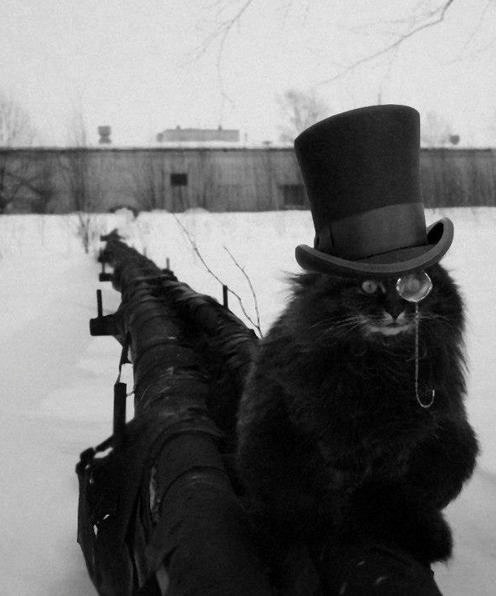
\includegraphics[scale=0.3]{cat}
\end{center}
\end{figure}
\newpage
\section{Tables}
\begin{center}
\begin{table}[!h]
\caption{Our First Table}
\begin{tabular}[!h]{c | c | c | c }
Subject & Difficulty & Fun & Usefulness\\ \hline
Econometrics & 10 & 10 & 10\\
Finance & 8 & 9 & 10\\
Macroeconomics & 9 & 7 & 9\\
Microeconomics & 7 & 4 & 1\\
\end{tabular}
\end{table}
\end{center}
\section{References}
 \bibliographystyle{plain}
This is our first reference \cite{OlmoPouliot}
\bibliography{myfirstbib}
\end{document}

